\documentclass[10pt,aspectratio=169,handout]{beamer}

\usepackage[utf8]{inputenc}
\usepackage[ngerman]{babel}
\usepackage{utopia}
\usetheme{Darmstadt}
\usecolortheme{default}
\usepackage{xcolor}
\usepackage{graphicx}
\usepackage{amsmath}
\usepackage{amsthm}
\usepackage{amssymb}
\usepackage{amsfonts}
\usepackage{mathtools}
\usepackage{dsfont}
\usepackage{hyperref}
\usepackage[most]{tcolorbox}
\usepackage{tikz}
\usepackage{adjustbox}
\usepackage{mathrsfs}
\usepackage{minted}
\usetikzlibrary{cd}
\usetikzlibrary{positioning}
\usetikzlibrary{calc}
\usetikzlibrary{arrows.meta}
\setbeamertemplate{theorems}[numbered]
\setbeamertemplate{navigation symbols}{}
\newtranslation[to=ngerman]{Theorem}{Satz}
\def\C{\mathbb{C}}
\def\R{\mathbb{R}}
\def\Q{\mathbb{Q}}
\def\N{\mathbb{N}}
\def\Z{\mathbb{Z}}
\def\cA{\mathcal{A}}
\definecolor{LightGray}{gray}{0.9}


\begin{document}

\title{Principles of Machine Learning: Exercise 3}
\date{04.12.2023}
\author{Alina Pollehn (3197257), Julian Litz (3362592), Manuel Hinz (3334548)\\
    Felix Göhde (3336445), Felix Lehmann (3177181), Caspar Wiswesser (3221493)\\
    Adrian Köring (3347785), Greta Günther (3326765), Linus Mallwitz (3327653)\\
    Niklas Mueller-Goldingen (3363219), Jennifer Kroppen (2783393)}

\begin{frame}
    \maketitle
\end{frame}

\section{Exercise 3.1}

\begin{frame}

    \frametitle{Implementation of exercise 3.1}

    outer difference: 
    \inputminted[bgcolor=LightGray,fontsize=\small]{python}{code/diffMatrix.py}

    outer product: 
    \inputminted[bgcolor=LightGray,fontsize=\small]{python}{code/prodMatrix.py}
    
    for general operators:
    \inputminted[bgcolor=LightGray,fontsize=\small]{python}{code/operatorMatrix.py}
    
\end{frame}

\section{Exercise 3.2}

\begin{frame}

    \frametitle{Implementation of exercise 3.2.1}
    
        Linear kernel matrix $K(u,v|\alpha)\in \R^{n_u\times n_v}$
        \[[K]_{ij}=\alpha u_i v_j\]
        \inputminted[bgcolor=LightGray,fontsize=\small]{python}{code/linearMatrix.py}


\end{frame}

\begin{frame}

    \frametitle{Implementation of exercise 3.2.2}
    
        gaussian kernel matrix $K(u,v|\alpha,\sigma)\in \R^{n_u\times n_v}$
        \[[K]_{ij}=\alpha \exp\left(-\frac{(u_i-v_j)^2}{2\sigma^2}\right)\]
        \inputminted[bgcolor=LightGray,fontsize=\small]{python}{code/gausMatrix.py}

\end{frame}

\section{Exercise 3.3}

\begin{frame}
    \frametitle{Sampling from a linear kernel matrix}

    Sampling 5 vectors twice yields

    \inputminted[bgcolor=LightGray,fontsize=\small]{python}{code/linear_sampling.py}

    \begin{minipage}{0.49\textwidth}
        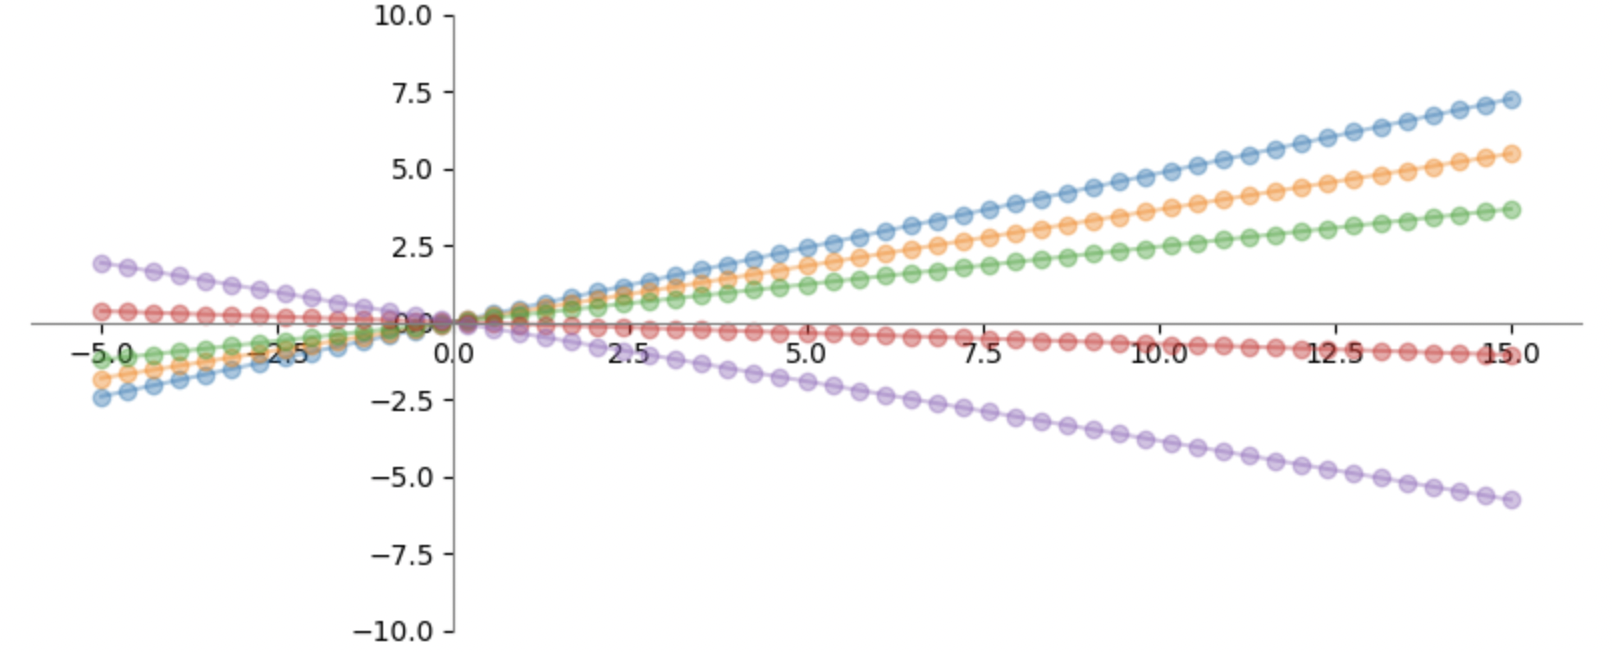
\includegraphics[width=\textwidth]{images/ex3.3.1a.png}
    \end{minipage}
    \begin{minipage}{0.49\textwidth}
        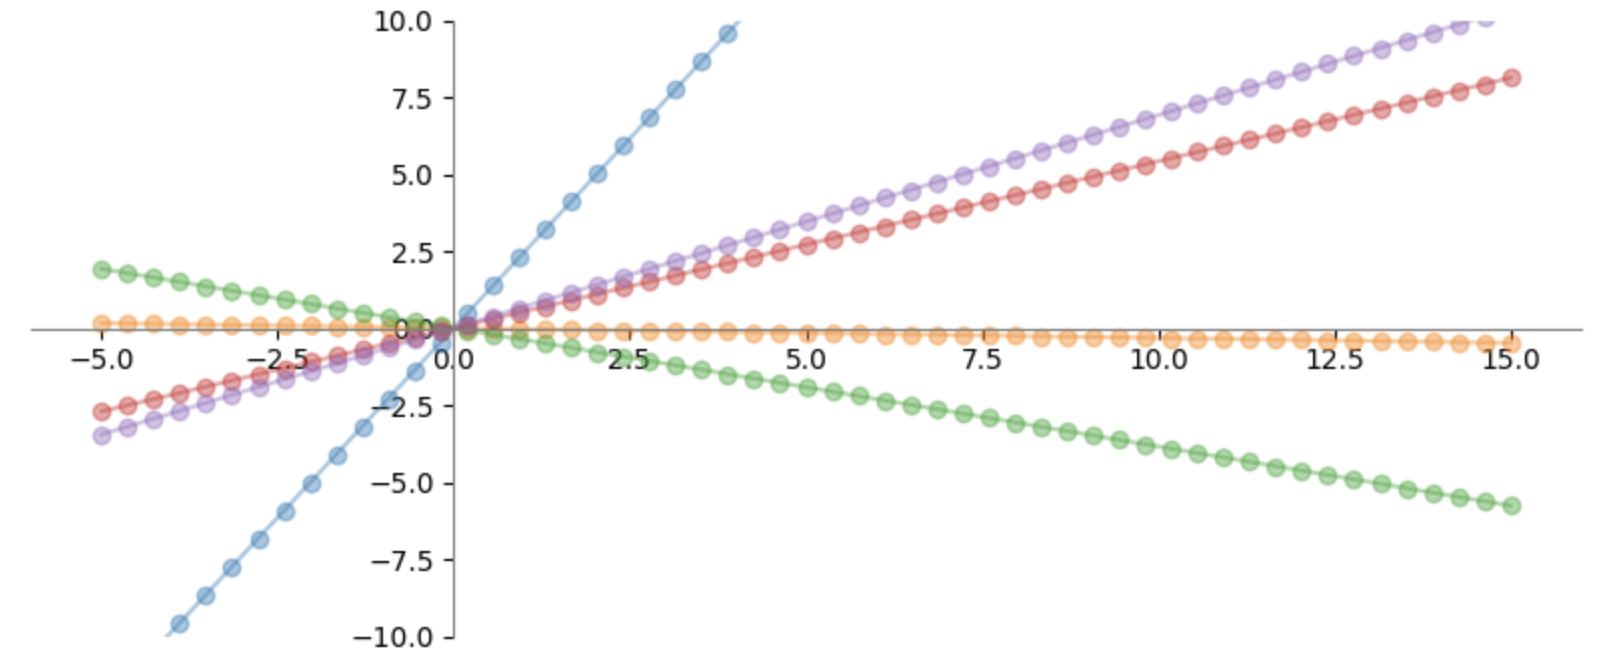
\includegraphics[width=\textwidth]{images/ex3.3.1b.png}
    \end{minipage}

    Keep in mind, that these results are random and will look different each time.
    Outliers, as seen in the second image, are quite common.

\end{frame}

\begin{frame}
    \frametitle{Sampling from a gaussian kernel matrix}

    Sampling 5 vectors twice yields

    \inputminted[bgcolor=LightGray,fontsize=\small]{python}{code/gaussian_sampling.py}

    \begin{minipage}{0.49\textwidth}
        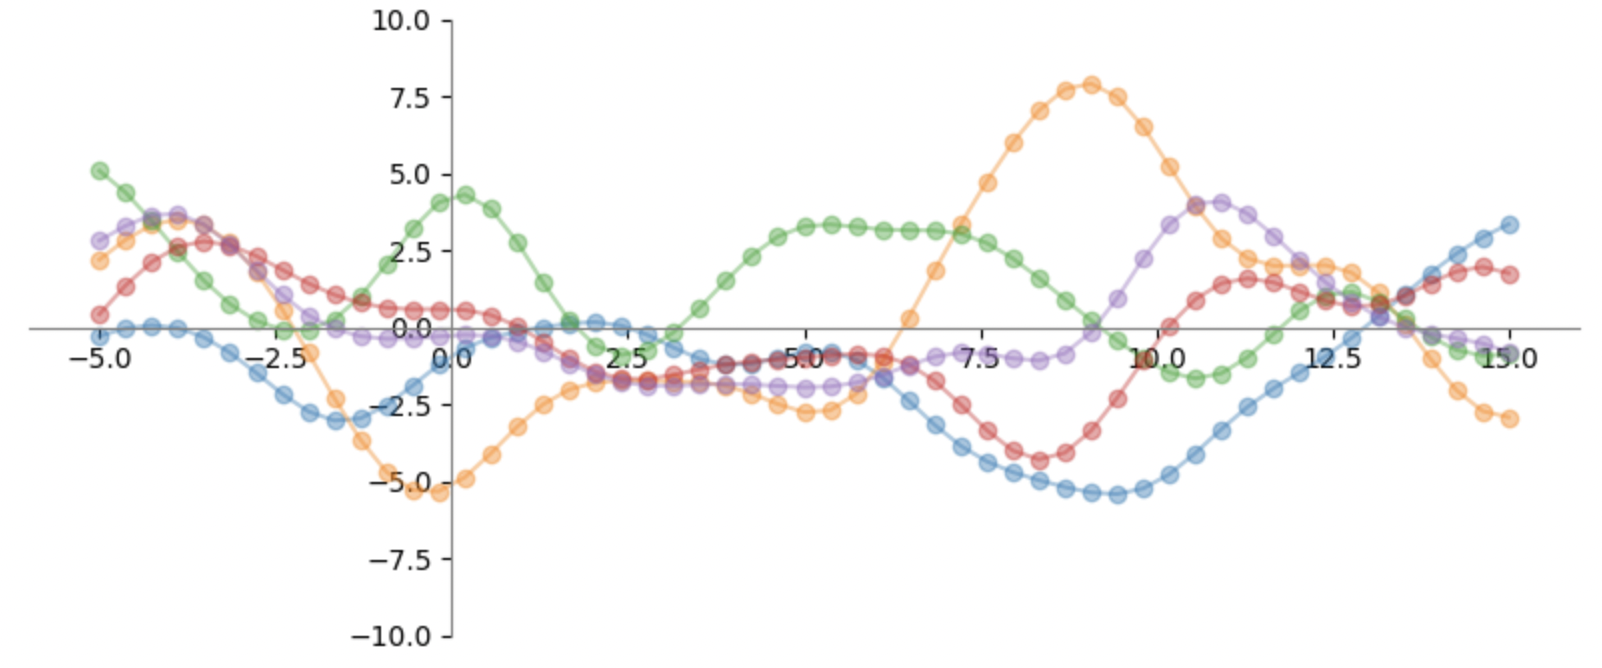
\includegraphics[width=\textwidth]{images/ex3.3.2a.png}
    \end{minipage}
    \begin{minipage}{0.49\textwidth}
        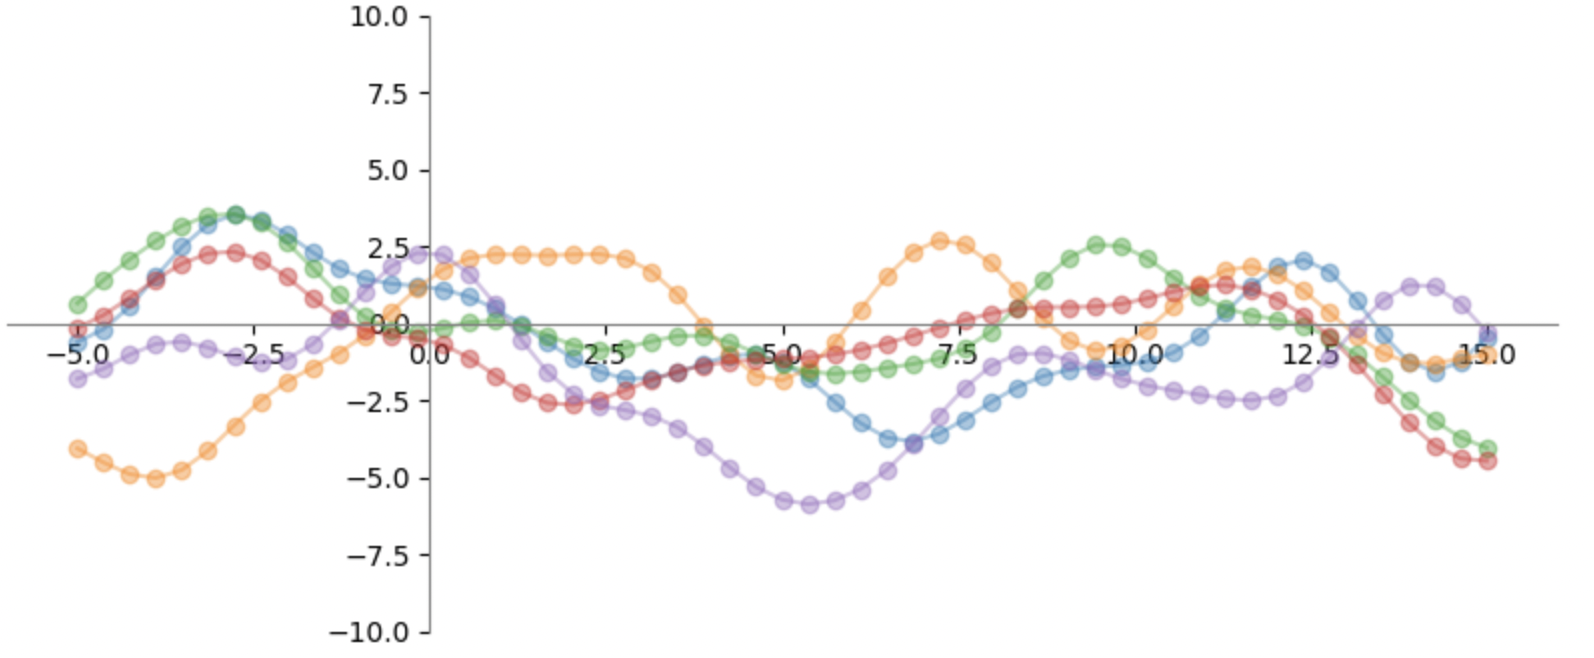
\includegraphics[width=\textwidth]{images/ex3.3.2b.png}
    \end{minipage}

    Keep in mind, that these results are random and will look different each time

\end{frame}



\end{document}
